\chapter{Fundamentals}\label{ch:methodology} %/ State of the art

The following chapter outlines the fundamentals of the methods used in this work.
First, the preprocessing of the data is described in \autoref{sec:preprocessing}.
Then, the different similarity measurements are introduced in \autoref{sec:similarity-measurement}.
Afterwards, a variety of ways to generate numerical representations of textual data is outlined in \autoref{sec:embeddings}.
Then, \autoref{sec:clustering} presents multiple clustering methods.
The database applied is described in \autoref{sec:db}.
Finally, the libraries used to implement the web application are introduced in \autoref{sec:BE_flask} and \autoref{sec:FE_angular}.



\section{Preprocessing}\label{sec:preprocessing}

Similar to other \ac{ml} domains, \ac{nlp} requires preprocessing of the data.
Usually, textual data contains irrelevant information and noise.
Hence, preprocessing improves the performance and the results \cite{clusteringDocs2020}.
The next sections describe a selection of the preprocessing steps applied in this work.


\subsection{Tokenization}\label{subsec:tokenization}

\textit{Tokenization} is the process of splitting a text into smaller pieces, so-called \textit{tokens}.
Tokens can be words and punctuation marks \cite{nlp-book2009}.
However, the definition of a token depends on the application.
For instance, certain tokenization implementations may identify tokens as subsequent series of non-whitespace characters omitting all numbers and punctuation marks \cite{IR2011}.

% \textit{Chunking} is the process of splitting a text into smaller pieces, so-called \textit{chunks}.
% A chunk is a sequence of tokens, e.g. words, in a text \cite{nlp-book2009}.
% Chunks do not overlap.
% According to \citeauthor{nlp-book2009}, chunkers produce their pieces by following a set of rules, e.g., grammar rules.

\subsection{Stemming}\label{subsec:stemming}

In order to avoid language inflections, i.e. treating words with similar meanings differently, stemming is applied \cite{clusteringDocs2020}.
According to \citeauthor{nlp-book2009}, \textit{stemming} is the process of striping off any affixes, i.e. prefixes and suffixes \cite{IR2011}, 
from a word and returning the stem.
Different types of stemmers are better suited for certain applications than others.
Hence, the choice of the stemmer depends on the application.

% For instance, the \textit{Porter Stemmer} performs well for English texts \cite{nlp-book2009, clusteringDocs2020}.
% It is predominantly used for the normalization of inflected forms.
% The \textit{Porter Stemmer} is an algorithmic stemmer, 
% i.e. it applies a set of rules to a word to produce the stem and thus, does not use a dictionary \cite{IR2011, clusteringDocs2020}.

\subsection{Lemmatization}\label{subsec:lemmatization}

Stemming and lemmatization are used to reduce the vocabulary size \cite{clusteringDocs2020}.
By ensuring the resulting stem is a valid word, the process of stemming is called \textit{lemmatization} \cite{nlp-book2009}.
Some implementations of lemmatizers only stem words if the result is in its dictionary.
Since lemmatizers validate the result prior to returning it, they are usually slower than stemmers \cite{nlp-book2009}.

The \textit{WordNetLemmatizer} from the \texttt{nltk} package requires a vocabulary. % \cite{clusteringDocs2020}.
According to \citeauthor{clusteringDocs2020}, it is frequently used for English texts.
It considers not only the meaning of words, but also the order of the words \cite{clusteringDocs2020}.


\subsection{Stop-Word-Removal}\label{subsec:stop-word-removal}

Omitting words that are not relevant to the context of the text is called \textit{stop-word-removal}.
Stop words not only depend on the domain but also the language \cite{IR2011}.


\subsection{Lower case}\label{subsec:lower-case}

Words with capital letters are converted to lowercase.



\section{Similarity Measurement}\label{sec:similarity-measurement}

Since embeddings represent texts as vectors, they not only facilitate human interpretability of relationships between texts using 
the text's respective point in a $N$-dimensional space, but also enable the use of similarity measures to quantify the similarity between texts.
A similarity measure defines a metric to quantify the similarity between two texts \cite{IR2011, euclidean_l2_norm2015}.

There are several similarity measures, such as the dot product quantifying the number of shared tokens of two texts, 
the (soft) cosine similarity, which is the normalized dot product and calculates the angle between two vectors, 
and many more \cite{IR2011, euclidean_l2_norm2015, HfsentTrans2019}.
The following section describes a few of the metrics usable for similarity measurement.


\subsection{Euclidian distance}\label{subsec:euclidian-distance}

The \textit{euclidian distance} is a distance measure.
In order to measure the distance between two points in a $N$-dimensional space, 
the root of the sum of squared distances between the respective values of every dimension is calculated.
The distance function Euclidean (L2) norm is given in \autoref{eq:euclidian-distance} from \cite{euclidean_l2_norm2015}.
The points $x_1, x_2$ correspond to objects $d_1, d_2$.

\begin{equation}
    d_E(x_1,x_2) = \sqrt{\sum_{i=1}^{N}(x_1\left[ i \right] - x_2\left[ i \right])^2}
    \label{eq:euclidian-distance}
\end{equation}


\subsection{Cosine Similarity}\label{subsec:cosine-similarity}

In the traditional bag-of-words approach the texts are represented as vectors of \ac{tfidf} coefficients \cite{soft_cosine2017}.
Without further processing, the vector is of size $N$, $N$ being the number of different words of the texts \cite{soft_cosine2017}.
Hence, a vector represents its corresponding text in a $N$-dimensional space.
This space is called \ac{vsm} \cite{soft_cosine2014}.

The similarity between two texts is measured by the cosine of the angle between their respective vectors \cite{soft_cosine2014}.
The cosine similarity is defined in \autoref{eq:cosine-similarity} from \cite{soft_cosine2014}.
$a \cdot b = \sum_{i=1}^{N}a_{i}b_{i}$ is the dot-product.
The dot-product is normalized with $\left\| x \right\| = \sqrt{x \cdot x}$ to unit Euclidean length \cite{soft_cosine2014}.
The cosine similarity is a value between $0$ and $1$ for positive values \cite{soft_cosine2014}.
According to \citeauthor{soft_cosine2014}, the formula has a time and space complexity of $O(N)$ for a pair of $N$-dimensional vectors.

\begin{equation}
    cosine(a,b) = \frac{a \cdot b}{\left\| a \right\| \times \left\| b \right\|} = \frac{\sum_{i=1}^{N}a_{i}b_{i}}{\sqrt{\sum_{i=1}^{N}{a}^2_{i}}\sqrt{\sum_{i=1}^{N}{b}^2_{i}}}
    \label{eq:cosine-similarity}
\end{equation}

The formula \autoref{eq:cosine-similarity} assumes that the vectors, which span the \ac{vsm} are orthogonal and thus, 
completely independent \cite{soft_cosine2014}.
However, in practical applications, this often is not the case \cite{soft_cosine2014}.


\subsection{Soft Cosine Similarity}\label{subsec:soft-cosine-similarity}

This similarity measure not only evaluates whether two texts consist of the same words but 
also takes into account the semantic (word-level) similarity or lexical relation of different words of the texts \cite{soft_cosine2017}.
Hence, it improves the shortcomings of the traditional cosine similarity measure, 
which assumes the tokens of the vocabulary are completely independent of each other \cite{soft_cosine2014}.

According to \citeauthor{soft_cosine2014}, in order to model this additional information, more dimensions are added to the \ac{vsm}.
These dimensions can be obtained, for instance, by multiplying the mean of two features of one vector with the similarity between them \cite{soft_cosine2014}.
The similarity can be calculated by using Levenshtein distance for e.g., n-grams, i.e. the number of operations necessary to convert one string into another, 
or using a dictionary of synonyms \cite{soft_cosine2014}.

Since this approach no longer assumes that different words are independent of each other, 
the basis vectors which span the \ac{vsm} are no longer orthogonal \cite{soft_cosine2014}.
The formula for the soft cosine similarity is defined in \autoref{eq:soft-cosine-similarity} from \cite{soft_cosine2014}.
The similarity $s_{ij}$ between the $i$-th and $j$-th basis vector is obtained using a similarity measure, such as synonymy \cite{soft_cosine2014}.

\begin{equation}
    soft\_cosine(a,b) = \frac{\sum_{i=1}^{N}\sum_{j=1}^{N}s_{ij}a_{i}b_{j}}{\sqrt{\sum_{i=1}^{N}\sum_{j=1}^{N}s_{ij}a_{i}a_{j}}\sqrt{\sum_{i=1}^{N}\sum_{j=1}^{N}s_{ij}b_{i}b_{j}}}
    \label{eq:soft-cosine-similarity}
\end{equation}

According to \citeauthor{soft_cosine2017}, the similarity between two texts is non-zero as soon as they share related words \cite{soft_cosine2017}.
If there is no similarity between different features, 
the soft cosine similarity from \autoref{eq:soft-cosine-similarity} is equal to the cosine similarity from \autoref{eq:cosine-similarity}.
The time and space complexity of the soft cosine similarity is $O(N^2)$ \cite{soft_cosine2014}.

In order to reduce the complexity, \citeauthor{soft_cosine2014} propose to use a sparse similarity matrix which only stores $s_{ij} > t$, 
$t$ being a threshold \cite{soft_cosine2014}.


\section{Embeddings}\label{sec:embeddings}

Usually, \ac{ml} techniques require textual inputs to be converted to embeddings \cite{SentRep2014}.
Embeddings are numerical representations of words, sentences or texts.
They can be used to present the textual data as real-valued vectors in a \ac{vsm}.
A \ac{vsm} is a $N$-dimensional space \cite{soft_cosine2014}.
%Each dimension of a \ac{vsm} corresponds to an index term, which is dependent on the embedding model.
%Every document embedding dimension explains the importance of the corresponding index term to the document.
\acp{vsm} are commonly used due to their conceptual simplicity and because spatial proximity correlates with semantic proximity 
\cite{tfidf2008, UniversalSentEnc2018, HfsentTrans2019, Top2Vec2020}.
Representations in a \ac{vsm} can improve the performance in \ac{nlp} tasks \cite{SkipGram2013}.
% According to \citeauthor{tfidf2008}, when representing text the first step is indexing, i.e.\ assigning indexing terms to the document.
% The second task is to assign weights to the terms that correspond to the importance of the term in the document.
% The weights assigned depend on the model.

The following section outlines the fundamentals of a selection of embeddings.
Let a corpus of documents be denoted $D= \left\{d_1, d_2, ..., d_M  \right\}$ 
and a sequence of terms $w_{ij}$ or so-called document $d_i = \left\{w_{i1}, w_{i2}, ..., w_{iV}  \right\}$, 
$V$ being the length of the vocabulary, 
i.e.\ set of distinct words \cite{clusteringDocs2020}, and $j \in [0, V]$.


\subsection{\acl*{tfidf}}\label{subsec:tfidf}

\ac{tfidf} provides a numerical representation of a word in a document \cite{clusteringDocs2020}.
Let a corpus of documents be denoted $D= \left\{d_1, d_2, ..., d_M  \right\}$, $M$ being the total number of documents in the corpus. 
Let a sequence of terms $w_{j} \in V$ be denoted a document $d_i = \left\{w_{1}, w_{2}, ...\right\}$, 
$V$ being the vocabulary, 
i.e.\ set of distinct words \cite{clusteringDocs2020}.

The \ac{tfidf} model considers the frequency $f_{w_{j}, d}$  of a word $w_{j}$ in a document $d$ and the frequency of a word in the whole corpus. 
The frequency $f_{w_{j}, d}$ is defined in \autoref{eq:tfidf_frequency}, $w'_j$ being the number of occurrences of $w_j$ in $d$.

\begin{align}
    f_{w_{j}, d} &= \frac{w'_{j}}{\sum_{k \in d} w'_k}\label{eq:tfidf_frequency}\\
    TFIDF(w_{j}, d, D) &= TF(w_{j}, d) \cdot IDF(w_{j}, D)\label{eq:tfidf_calculation}\\
    TF(w_{j}, d) &= f_{w_{j}, d}\label{eq:tf_calculation}\\
    IDF(w_{j}, D) &= \log_2\frac{M}{M_{j}}\label{eq:idf_calculation}
\end{align}

\ac{tfidf} is calculated using \autoref{eq:tfidf_calculation} from \cite{clusteringDocs2020}.
Each entry of a \ac{tfidf} embedding vector represents the \ac{tfidf} value of a word in a document.
Hence, the embedding vector is of the same length as the vocabulary of the corpus.
The \ac{tf} is determined utilizing \autoref{eq:tf_calculation}, 
whereas the \ac{idf} is computed by \autoref{eq:idf_calculation}, 
$M_{j}$ being the number of documents the term $w_{j}$ appears in.

\ac{idf} measures the importance of a term $w_{j}$ in the corpus of documents $D$
under the assumption that a term's importance to the data corpus is inversely proportional to its occurrence frequency \cite{tfidf2008}.
In other words: Terms which appear in many documents are not as important and thus, weighted less than document-specific terms. 
The calculation of \ac{tf} and \ac{idf} is visualized exemplary in \autoref{fig:tfidf-calculation}.


\begin{figure}[!htb] % htp = hier (h), top (t), oder auf einer eigenen Seite (p).
    \centering
    \includesvg[width=0.7\textwidth]{images/embeddings/tfidf/tfidf.svg}
    \caption[Exemplary calculation of \acs*{tf} and \acs*{idf} values]{
        Exemplary calculation of \acs*{tf} and \acs*{idf} for a document corpus $D$: 
        \acs*{tf} only considers the documents of interest while 
        \acs*{idf} incorporates the importance of the word with respect to $D$.
    }
    \label{fig:tfidf-calculation}
\end{figure}

%According to \citeauthor{tfidf2008}, the computation complexity of \ac{tfidf} embeddings is $O(V \cdot M)$.
\ac{tfidf} has several drawbacks \cite{clusteringDocs2020,tfidf2008}:
\begin{itemize}
    \item \ac{tfidf} does not consider semantic similarities between words.
    \item \ac{tfidf} does not take into account the order of words in a document.
    \item \ac{tfidf} often produces high dimensional representations which have to be postprocessed to reduce their dimensionality, e.g., by using \ac{pca}.
    %\item The embeddings are not derived from a mathematical model of term distribution and thus, are occasionally criticised as not well reasoned.
\end{itemize}

% TODO: advantages of tfidf?

\subsection{\ac{d2v}}\label{subsec:doc2vec}

Another term used for \ac{d2v} is \textit{Paragraph Vector} \cite{clusteringDocs2020, SentRep2014}.
\ac{d2v} addresses the problems of \ac{tfidf} by encoding texts as $N-$dimensional vectors learnt using the words' context \cite{clusteringDocs2020}.
Hence, it preserves semantic similarities between words and encodes linguistic regularities and patterns \cite{SkipGram2013}.
% According to \citeauthor{clusteringDocs2020} and \citeauthor{SentRep2014}, 
% \ac{d2v} learns continuous distributed vector representations for pieces of the text.
The model handles inputs of different dimensions and thus, tokens can be sentences, paragraphs or documents.

\ac{d2v} is an adaption of the \ac{w2v} model, which maps words into a \ac{vsm} \cite{clusteringDocs2020}.
Both approaches assume that words appearing in similar contexts are semantically similar. %\cite{clusteringDocs2020}.
The \ac{w2v} embedding is obtained using a shallow \ac{nn}, i.e. the \ac{nn} has only one hidden layer.
The embeddings are created by the hidden layer.
There are two approaches to designing the architecture of the \ac{nn}:
\begin{itemize}
    \item \ac{pvdm}: 
        Predicts a word given a context \cite{SentRep2014, WordRep2013}.
    \item \ac{pvdbow}: 
        Predicts the context given a word \cite{EmbDist2015, SkipGram2013, SentRep2014}.
\end{itemize}

% \begin{equation}
%     \frac{1}{T}\sum_{t=k}^{T-k}\text{log}(p(w_t | w_{t-k}, ..., w_{t+k}))
%     \label{eq:word2vec-cbow}
% \end{equation}

\begin{figure}%
    \centering
    \subfloat[\centering \ac{cbow} architecture cf. \cite{WordRep2013}.]
    {{\includesvg[width=7cm]{images/embeddings/doc2vec/CBOW.svg}}}%
    \qquad
    \subfloat[\centering \ac{pvdm} architecture cf. \cite{SentRep2014}.]
    {{\includesvg[width=6cm]{images/embeddings/doc2vec/PV-DM.svg} }}%
    \caption[\ac{cbow} and \ac{pvdm} architecture]{Both approaches predict the centre word using the context.
    \ac{pvdm} is an adaption of \ac{cbow} to work on a set of documents or paragraphs instead of words.
    }%
    \label{fig:pvdm}%
\end{figure}
 
% context to center word
\ac{pvdm} extends \ac{cbow} to work on a corpus of documents instead of on a set of words \cite{clusteringDocs2020}:
As usual, vectors representing the words are obtained using the \ac{cbow} model.
\ac{cbow} has a single-layer architecture \cite{glove2014}. %based on the inner product between two word vectors \cite{glove2014}.
%Given training words $ w_{1}, ..., w_{T}$, the objective of the \ac{w2v} model \ac{cbow} is to maximize the average log probability in 
%\autoref{eq:word2vec-cbow} from \cite{SentRep2014}.
The word vectors can be concatenated, averaged or summed up \cite{SentRep2014}.
Each document is mapped to a vector using an additional document-to-vector matrix.
Both document and word vectors are initialized randomly, but trained to convey meaning in terms of semantic differentiation.
In order to train the model, center words are predicted using the context.
The context consists of words within a sliding window and their document, respectively represented as vectors \cite{SentRep2014}.
The document vector is added to incorporate the document's topic and thus, acts like a memory \cite{SentRep2014, Top2Vec2020}.
\citeauthor{SentRep2014} concatenate the document vector to the word vectors.
The resulting vector is the prediction of the central word.
The approaches are displayed in \autoref{fig:pvdm}.

According to \citeauthor{SentRep2014}, both \ac{cbow} and \ac{pvdm} are trained using stochastic gradient descent and backpropagation.
They also state that the document vectors are unique, while the word vectors are shared across the whole corpus. 

\begin{figure}%
    \centering
    \subfloat[\centering Skip-gram architecture cf. \cite{WordRep2013}.]
    {{\includesvg[width=7cm]{images/embeddings/doc2vec/Skip-gram.svg}}}%
    \qquad
    \subfloat[\centering \ac{pvdbow} architecture cf. \cite{SentRep2014}.]
    {{\includesvg[width=4.5cm]{images/embeddings/doc2vec/PV-DBOW.svg} }}%
    \caption[Two \ac{pvdbow} architectures]{Both approaches predict the context.
    \ac{pvdbow} is an adaption of Skip-gram to work on a set of documents or paragraphs instead of words.
    }%
    \label{fig:pvdbow}%
\end{figure}
% center word to context
The \ac{pvdbow} approach is the adaption of the \ac{w2v} algorithm Skip-Gram and predicts the context 
given the document \cite{SentRep2014}.
The approaches are displayed in \autoref{fig:pvdbow}.
%According to \citeauthor{SentRep2014}, the 


% paper widerspricht sich
%According to \citeauthor{clusteringDocs2020}, the \ac{doc2vec} model's performance is influenced quality of the preprocessing.
%If for instance, the stemmer assigns words with different meaning to the same root, there is a degradation in performance.

\subsection{\acl*{use}}\label{subsec:univ-sent-encoder}

\citeauthor{UniversalSentEnc2018} have published their \acf{use} model on TensorFlow Hub.
They propose two architectures, one based on a Transformer and one based on a \ac{dan} \cite{UniversalSentEnc2018}.
Both models' input is a lowercase tokenized string.
Their output is a 512-dimensional vector.

% Transformer
The transformer model is more accurate and more complex than the \ac{dan} model \cite{UniversalSentEnc2018}.
The transformer's (self) attention is used to compute context-aware word embeddings, which consider both the word order and their semantic identity.
Since a sequence of word embeddings of a sentence produces embeddings of different dimensions, the approach postprocesses the word embeddings.
A sentence vector is obtained by computing the element-wise sum of the word embeddings 
and normalizing the result by dividing by the square root of the sentence length.

% DAN
The \ac{dan} model receives real-valued embeddings of words and bi-grams as input.
A bi-gram is a tupel of two subsequent words in a text \cite{nlp-book2009}, for instance, \textit{(red, wine), (wine, tastes), (tastes, good)}.
The embeddings can be obtained from the text strings using models such as the \ac{bow} model \cite{UniversalSentEnc-dan-input-emb}.
They are averaged and subsequently passed to a feedforward \ac{dnn} \cite{UniversalSentEnc2018}.
The architecture of the \ac{dan} model is depicted in \autoref{fig:use_dan}.

\begin{figure}[!htp] % htp = hier (h), top (t), oder auf einer eigenen Seite (p).
    \centering
    \includesvg[width=0.9\textwidth]{images/embeddings/universal_sentence_encoder/DAN.svg}
    \caption[Architecture of \acs*{use}]{Architecture of the \acs*{dan} model used for \acs*{use} based on the textual description from \cite{inferSent2018}.
    The input words and bi-grams $(w_1, w_2, ..., w_N)$ are embedded.
    The embeddings are averaged and subsequently passed to a feedforward \acs*{dnn}, which produces a 512-dimensional sentence embedding.
    }
    \label{fig:use_dan}
\end{figure}

% dataset
The models are trained on both unsupervised training data, e.g., Wikipedia, and a supervised training dataset, i.e.\ \ac{snli} \cite{UniversalSentEnc2018, HfsentTrans2019}.
The unsupervised training task is to predict the context given an input, i.e.\ Skip-Gram like tasks.
The supervised training task is classification \cite{UniversalSentEnc2018}.

% complexity
%The transformer model is more complex than the \ac{dan} model.
% The transformer model complexity is $O(n^2)$, whereas the \ac{dan} model complexity is $O(n)$, 
% $n$ being the number of words in the sentence \cite{UniversalSentEnc2018}.
% % memory usage
% The memory usage of both models is equivalent to their complexity.
% \citeauthor{UniversalSentEnc2018} state that \ac{dan}'s memory usage is dominated by the parameters used to store the embeddings of the uni- and bi-grams.
% Moreover, the transformer model only stores the uni-gram embeddings and thus, can require less memory than \ac{dan} for short sentences \cite{UniversalSentEnc2018}.

\subsection{\infersent{}}\label{subsec:inferSent}

% general
\infersent{} is a sentence embedding method trained in a supervised manner on the \ac{snli} dataset \cite{inferSent2018, HfsentTrans2019}.
The trained model is transferable to other tasks.
% Bi-LSTM as sentence encoder
\citeauthor{inferSent2018} compare multiple architectures in their work.
The \ac{bilstm} architecture with max pooling which was found to be the best option for the sentence encoder 
is depicted in \autoref{fig:infersent_bilstm} \cite{inferSent2018}.

\begin{figure}[!htb] % htp = hier (h), top (t), oder auf einer eigenen Seite (p).
    \centering
    \includesvg[width=0.9\textwidth]{images/embeddings/infersent/Infersent.svg}
    \caption[Architecture of \infersent{}]{Architecture of the \acs*{bilstm} model with max pooling used for \infersent{} cf. \cite{inferSent2018}.
    The input sentence $(w_1, w_2, ..., w_T)$ is read from both directions by a forward and a backward \acs*{lstm} 
    producing $\overrightarrow{h_t}$ and $\overleftarrow{h_t}$ respectively.
    After concatenating $\overrightarrow{h_t}$ and $\overleftarrow{h_t}$ to $h_t$, max pooling is applied.
    The output is a fixed-sized embedding.
    }
    \label{fig:infersent_bilstm}
\end{figure}

% LSTM
A \ac{lstm} is a \ac{rnn} that is capable of learning long-term dependencies.
\acp{rnn} have closed loops, i.e.\ feedback connections between the nodes \cite{rnn_book2001}.
In other words, 
a \ac{lstm} is able to remember information as a so-called \textit{state}.
Certain \ac{lstm} mechanisms control whether the current state is deleted, whether new data is saved and 
to what degree the current state contributes to the current input processed in the node.
Hence, \ac{lstm} nodes are not only influenced by former outputs but also by their state.
Since the \ac{lstm} computes different numbers of hidden vectors $h_t$ depending on the length of a sentence, 
a max pooling layer is applied to the hidden vectors which selects the maximum value for a patch of the hidden vectors.

% Bi-LSTM
According to \citeauthor{HfsentTrans2019}, \infersent{} consists of a single \ac{bilstm} layer \cite{HfsentTrans2019}.
Given a sentence $(w_1, w_2, ..., w_T)$ of $T$ words, the \ac{bilstm} architecture computes the hidden representations $h_t$ for each word $w_t$.
The hidden representation $h_t$ is the concatenation of the forward and backward hidden vectors $\overrightarrow{h_t}$ and $\overleftarrow{h_t}$.
$\overrightarrow{h_t}$ and $\overleftarrow{h_t}$ are produced by a forward and backward \ac{lstm} respectively.
Hence, the sentence is read from both directions and thus, considers past and future context.

\subsection{\acl*{sbert}}\label{subsec:hf-sent-ransformers}

\ac{sbert} is an enhancement of \ac{bert}.
% BERT
\ac{bert} is a pre-trained transformer network.
It predicts a target value, for i.e. classification or regression tasks, based on two input sentences \cite{HfsentTrans2019}.
The input sentences are separated by a special token \texttt{[SEP]}.
The base model applies multi-head attention over 12 transformer layers, whereas the large model applies multi-head attention over 24 transformer layers.
The final label is derived from a regression function, which receives the output of the $12^\text{th}$ or $24^\text{th}$ layer, respectively.
\citeauthor{HfsentTrans2019} state that \ac{bert} is not suitable for specific pair regression tasks, 
since the number of input sentence combinations is too big.
Another shortcoming of \ac{bert} is that it does not produce independent embeddings for single sentences.
Moreover, \citeauthor{HfsentTrans2019} found that common similarity measurements, for instance, the ones discussed in \autoref{sec:similarity-measurement}, 
do not perform well on sentence embeddings produced by \ac{bert} \cite{HfsentTrans2019}.

% SBERT
\ac{sbert} provides fixed-sized embeddings for single sentences \cite{HfsentTrans2019}.
It differs from \ac{bert} in terms of architecture, since it adds a pooling layer after the \ac{bert} model.
\citeauthor{HfsentTrans2019} compare different pooling strategies, such as using the output of the \texttt{CLS} (i.e. first) token, mean pooling and max pooling.
The architecture of a single \ac{sbert} network is depicted in \autoref{fig:sbert}.
In order to work with multiple input sentences at the same time, siamese and triplet network architectures, 
i.e. multiple \ac{bert} networks with tied weights, are constructed.
To perform classification or inference tasks layers are added on top of the \ac{sbert} network.
% training corpus
\ac{sbert} is trained on the \ac{snli} dataset.

\begin{figure}[!htb] % htp = hier (h), top (t), oder auf einer eigenen Seite (p).
    \centering
    \includesvg[width=0.7\textwidth]{images/embeddings/SBERT/SBERT.svg}
    \caption[Architecture of \ac{sbert}]{Architecture of \ac{sbert} cf. \cite{HfsentTrans2019}.
    \ac{bert} is extended by a pooling layer.
    The input is a sentence and the output is a fixed-sized embedding.
    }
    \label{fig:sbert}
\end{figure}

% performance
According to \citeauthor{HfsentTrans2019}, \ac{sbert} outperforms \infersent{} and \ac{use} on Semantic Textual Similarity tasks 
and on SentEval, which is an evaluation toolkit for sentence embeddings \cite{HfsentTrans2019}.
Moreover, due to \ac{sbert}'s transformer architecture, it is more computationally efficient than \ac{use} on \acp{gpu}.


\section{Topic Modelling}\label{sec:topic-modelling}

Since more and more textual data emerges, methods to analyse and extract information from texts become more important.
One of these methods is topic modelling.
%It is used to discover groups of words with similar meanings in a text corpus \cite{topic_modeling2015}.
A topic can be defined as a cluster of words that frequently occur together.
Subsequently, it is described by a probability distribution over a vocabulary.
A document can be represented by one or more topics. %and thus, can be created by a distribution over topics and a distribution over words given the topics.
%According to \citeauthor{topic_modeling2015}, topic models ignore the order of words in a document by relying on the bag-of-words assumption.
Common topic modelling algorithms include \ac{lda} \cite{topic_modeling2015}.


\subsection{\acl*{lda}}\label{subsec:latent-dirichlet-allocation}

\ac{lda} is a generative model, which recreates the original document word distributions with minimal error given the topics \cite{topic_modeling2015, Top2Vec2020}.
A discrete multinomial probability distribution over a vocabulary consisting of $W$ words is called a topic.
A document is a mixture of $K$ latent topics.
$K$ is defined a priori by the user.
Hence, each document from the document corpus $D$ is represented by specific topic probabilities.

The probability distribution learned by \ac{lda} only considers the statistical relationship of word occurrences in documents \cite{Topic2Vec2015}.
The content of a document can be described by the top $N$ words with the highest conditional probability given a topic \cite{Topic2Vec2015}.
Due to the fact that \ac{lda} considers high probability words to be informative, words 
that occur frequently are deemed important even though they might be uninformative in reality \cite{Top2Vec2020, Topic2Vec2015}.


\subsection{Top2Vec}\label{subsec:top2vec}

The approach \topTwovec{} was proprosed by \citeauthor{Top2Vec2020} \cite{Top2Vec2020}.
It addresses several problems of state-of-the-art topic modelling approaches, such as \ac{lda}.
Opposed to \ac{lda}, \topTwovec{} does not require the user to specify the number of topics $k$, 
i.e. it does not discretize the topic space into $k$ topics, 
and it does not require stop word removal or lemmatization.
Moreover, it considers the semantic meaning of words unlike \ac{lda}.
In contrast to \ac{lda}, \topTwovec{} only associates one topic with a document.

\begin{figure}%
    \centering
    \subfloat[\centering Skip-gram architecture cf. \cite{Topic2Vec2015}.]
    {{\includesvg[width=5.5cm]{images/topic_modelling/Skip-gram_Top2Vec.svg}}}%
    \qquad
    \subfloat[\centering \ac{cbow} architecture cf. \cite{Topic2Vec2015}.]
    {{\includesvg[width=5.5cm]{images/topic_modelling/CBOW_Top2Vec.svg} }}%
    \caption[Two learning architectures of \topTwovec{}]{Both learning architectures of \topTwovec{}.
    $w(t-2), w(t-1), w(t+1), w(t+2)$ are the context words of the centre word $w(t)$ of topic $z(t)$.
    }%
    \label{fig:top2vec_architectures}%
\end{figure}

% word2vec and doc2vec
\topTwovec{} is based on \ac{w2v} and \ac{d2v}.
The documents are embedded using \ac{pvdbow}.
There are two learning architectures adapted from \ac{w2v} to train the model, namely \ac{cbow} and Skip-gram \cite{Topic2Vec2015}.
They are depicted in \autoref{fig:top2vec_architectures}.
The Skip-Gram learning task is to predict the document a word came from \cite{Top2Vec2020, Topic2Vec2015}.
Similar to \ac{d2v}, \topTwovec{} not only embeds words and documents in the same feature space but also topics \cite{Top2Vec2020, Topic2Vec2015}.
The similarity between embeddings can be measured using the cosine similarity function \cite{Topic2Vec2015}.
\citeauthor{Top2Vec2020} regards each point in the \ac{vsm} as a topic, described by its nearest words.

% topics & clustering
\citeauthor{Top2Vec2020} states that topics are continuous and can be described by different sets of words \cite{Top2Vec2020}.
Hence, topic modelling is defined as the task of finding sets of informative words that describe a document.
Documents in dense areas of the topic space are considered to be about the same topic.
The density-based clustering algorithm \ac{hdbscan} is used to find these dense areas.
The topic vector is denoted as the centroid or average of the document vectors belonging to the topic.
\citeauthor{Top2Vec2020} has compared several topic vector definitions and found the arithmetic mean to be the best option \cite{Top2Vec2020}.
The number of topics is derived from the number of dense areas.
It is possible to merge topics to hierarchically reduce the number of topics found to any number of topics smaller than the number initially found.

% dimensionality reduction
In order to find topics, clusters of documents, i.e. dense areas, need to be identified.
The clustering algorithm \ac{hdbscan} is used to find these dense areas.
Since \ac{hdbscan} has difficulties finding dense clusters in high-dimensional data, 
the dimensionality reduction method \ac{umap} is applied \cite{Top2Vec2020}.
The steps of the topic modelling procedure \topTwovec{} are depicted in \autoref{fig:top2vec}.

% complexity
According to \citeauthor{Topic2Vec2015}, the complexity of \topTwovec{} is linear with the size of the dataset \cite{Topic2Vec2015}.

\begin{figure}[htp] % htp = hier (h), top (t), oder auf einer eigenen Seite (p).
    \centering
    \includesvg[width=0.7\textwidth]{images/topic_modelling/Top2Vec.svg}
    \caption{Procedure of topic modelling using \topTwovec{}.}
    \label{fig:top2vec}
\end{figure}



\subsection{\wordcloud{}s}\label{subsec:word-clouds}

A \wordcloud{} is a technique to visualize the most predominant words in a text \cite{topic_modeling2019}.
The size of a word correlates to its frequency or importance in the text.
However, a word does not have to be meaningful to appear large.
A \wordcloud{} does not provide information about the meaning or context of words and thus, 
one has to be careful when interpreting the results.


\section{Compression of data}\label{sec:compression}

According to \citeauthor{clusteringDocs2020}, a decomposition of data that preserves the inner structure in inherent clusters 
When data analysis techniques are applied to reasonably low-dimensional data the results usually improve.
Moreover, compressed data is less memory-consuming and often less difficult to interpret by humans 
since there are more methods to visualize low-dimensional data.
In the following two approaches to reduce the dimensionality of data are presented.

\subsection{\acl*{ae}}\label{subsec:autoencoder}

The idea of this approach is to find a meaningful low-dimensional version of the input.
The high-dimensional data is encoded into a low-dimensional representation using the encoder of an undercomplete \ac{ae} \cite{autoencoder2020}.
Hence, the output of the latent space corresponds to the input's embedding. 
The low-dimensional representation can be decoded into an approximation of the high-dimensional original using the decoder of the \ac{ae}.

\begin{figure}[!htb] % htp = hier (h), top (t), oder auf einer eigenen Seite (p).
    \centering
    \includesvg[width=0.4\textwidth]{images/embeddings/autoencoder/AE.svg}
    \caption[Structure of an \ac{ae}]
    {Structure of an \ac{ae} cf. \cite{autoencoder2020}}
    \label{fig:ae}
\end{figure}

An undercomplete \ac{ae} is a feed-forward \ac{nn}, which consists of an encoder and a decoder.
It learns efficient (non-correlated) encodings of the input data \cite{autoencoder2020}.
It is \textit{undercomplete} because the dimensionality of the hidden layer, or so-called hidden space, 
is lower than the dimensionality of the input layer \cite{seminar_ies}.
\textit{Feed-forward} means that the information flows from the input layer to the output layer \cite{seminar_ies}.
However, while training, the network employs backpropagation to update the parameters of the network \cite{seminar_ies}.

The \ac{ae}'s goal is to approximate the identity function $f_\theta(X) = X$ (trivial solution eliminated) for input $X$ and 
function parameters to be learned $\theta$ \cite{seminar_ies}.
The input and output layers have the same dimensionality.

% \begin{equation}
%     Z = f_E(W_\theta X + B_\theta)
%     \label{eq:encoder}
% \end{equation}

% The formulae for the encoder and the decoder are given in \autoref{eq:encoder} and in \autoref{eq:decoder}.
% The parameter $W_\theta$ is the weight, whereas $B_\theta$ is the bias.
% The activation functions $f_E$ and $f_D$ are possibly non-linear and thus, the \ac{nn} is capable of more than linear regression.
% $Z$ is the low-dimensional representation of the input $X$ and $X'$ is the reconstructed version of $Z$.

% \begin{equation}
%     X' = f_D(W_\theta Z + B_\theta)
%     \label{eq:decoder}
% \end{equation}

% The loss function $L$ is defined as the reconstruction error between the input $X$ and the output $X'$ \cite{seminar_ies}.
% In order to train the \ac{ae}, the loss function is minimized \cite{autoencoder2021}.


\subsection{\eigenfaces{}}\label{subsec:eigenface}

According to \citeauthor{eigenfaces1991}, the idea of \eigenfaces{} is inspired by information theory.
Opposed to former approaches in the domain of face recognition which relied on the classification of images based on a set of predefined facial features, such as distance between eyes,
\eigenfaces{} does not use predefined features \cite{eigenfaces1991}.
The goal of this approach is to represent images using a smaller set of image features, i.e. compression to a lower-dimensional feature space, 
such that it is possible to distinguish between the images \cite{eigenfaces1991, eigenfaces2013}.
These features do not necessarily correspond to human facial features \cite{eigenfaces1991}.
Similar pictures, i.e. of the same person, should lie on a manifold in the lower-dimensional feature space \cite{face-recognition2008}.
The decomposition of input images not only reduces the complexity but also facilitates modelling probability density of a face image \cite{face-recognition2008}.

% input image
% greyscale
The greyscale input images are two-dimensional arrays of numbers: $\textbf{x} = \left\{ x_i, i \in \textbf{S} \right\}$, $\textbf{S}$ being a square lattice \cite{eigenfaces1997, eigenfaces1991}.
The images are reshaped to an one-dimensional array $\textbf{x} = \left[x_1, x_2, ..., x_n  \right]^{T} \in \mathbb{R}^{n}$, 
where $n = \left\| \textbf{S} \right\|$ and $\mathbb{R}^{n}$ is the $n$-dimensional euclidean space \cite{eigenfaces1997}.
% background
Some authors stress that the background is removed to omit values outside the face area \cite{eigenfaces1991}.
% dimension
In literature, typically, the original images' dimension is 512x512 \cite{eigenfaces1991}/ 64x64 \cite{face-recognition2020}, 
whereas the projected images' dimension is 16x16 \cite{eigenfaces1991}/ 250 \cite{face-recognition2020}.
% normalization/ centering
\citeauthor{eigenfaces1991} stress that the data should be normalized, i.e. centred: 
$\Phi_{k} = \mathbf{x}_{k} - {\psi }$. 
$\Phi_{k}$ being the difference of the $k$-th training image and the average image $\psi = \frac{1}{N}\sum_{k=1}^{N}\textbf{x}_{k}$, $N$ being the number of training images.

% decomposition
The next step is to find an alternative lower-dimensional representation of the images, which preserves most of the information of the original image.
In mathematical terms, this decomposition can be expressed as 
$\textbf{x} = \sum_{i=1}^{n}\hat{x}_{i} \textbf{e}_{i}$, 
$\hat{x}_{i}$ being inner product of $\textbf{x}$ and $\textbf{e}_{i}$, 
$\textbf{e}$ being an orthogonal basis 
\cite{eigenfaces1997}.
If all basis vectors are used, the original image can be reconstructed using a linear combination of the basis vectors \cite{eigenfaces1991, face-recognition2020}.
The number of basis vectors is limited by the minimum of the training set size $N$ \cite{eigenfaces1991} and the number of pixels $n$ \cite{face-recognition2020}.
In order to compress the input from a $n-$ to a $m$-dimensional space, given $m \ll n$, only the first $m$ basis vectors are used.
The parameter $m$ is chosen such that $\hat{x}_{i}$ is small for $i \ge m$ \cite{eigenfaces1997}.
The compressed version of the image is denoted $\textbf{x} \simeq \hat{\textbf{x}} = \left[\hat{x}_{1}, \hat{x}_{2}, ..., \hat{x}_{m}  \right]^{T}$.
In other words: 
The compressed image is a vector of the first $m$ weights of the linear combination of weight and basis vectors used to transform the image back to the original space \cite{eigenfaces1991}.
The weights denote the position of the projection of the face images in the feature space or so-called face space spanned by the first $m$ basis vectors \cite{eigenfaces1991}.

% eigenfaces: KL base
In the context of \eigenfaces{} one basis used for decomposition is the \ac{kl} basis, i.e. \ac{pca} \cite{eigenfaces1997, eigenfaces1991}.
% source 1991, pg. 587: or fourier basis
According to \citeauthor{eigenfaces1997}, the \ac{kl} representation is optimal in the sense that it minimizes the \ac{rmse} between the original image and 
the compressed image calculated using $m < n$ orthogonal vectors.
The \ac{kl} basis consists of the eigenvectors of covariance matrix $\textbf{C} = E\left[ \textbf{x}\textbf{x}^{T} \right]$ of the input images $\mathbf{x}$ \cite{eigenfaces1997}.
% determine the number of components m
Since these eigenvectors can have facial features, they are called \textit{\eigenfaces{}}.
There are two approaches in the literature to determine the number of \eigenfaces{} $m$ used to compress the input images:
\begin{enumerate}[label=(\alph*)]
    \item The cumulative explained variance of the first $i \le n$ eigenvectors (sorted by eigenvalues $\lambda_i$) is calculated 
        \cite{eigenfaces1997, face-recognition2020, face-recognition2021}.
        The eigenvalues $\lambda_i$ can be interpreted as the amount of variance explained by the corresponding eigenvector $\textbf{e}_i$, which is equivalent to information or entropy.
        The user can choose how much variance, i.e. information, should be preserved, by choosing $m$ such that the explained variance is greater than a chosen threshold.
        \citeauthor{face-recognition2021} use a threshold of 90\%.
        A plot displaying the cumulative explained variance and a threshold of 90\% is shown in \autoref{fig:det_n_comp} (a).

    \item The number of \eigenfaces{} $m$ is chosen using the reconstruction error-complexity trade-off. % \cite{face-recognition2008}.
        The reconstruction error, i.e. the \ac{rmse} of the original image $X$ and the inverse transformed image $X'$ 
        calculated in \autoref{eq:rsme} for different values of $m$.
        The "elbow" point marks the point where the reconstruction error decreases only slightly for increasing $m$ and thus, is an indicator for the optimal $m$.
        A visualization of this approach is shown in \autoref{fig:det_n_comp} (b).
\end{enumerate}

\begin{equation}
    \text{RSME} = \sqrt{\frac{\sum_{i=1}^{N}(x_{i}-x'_i)^2}{N}}
    \label{eq:rsme}
\end{equation}
 
\begin{figure}%
    \centering
    \subfloat[\centering The cumulative explained variance of the first $i \le n$ eigenvectors (sorted by eigenvalues $\lambda_i$).]
    {{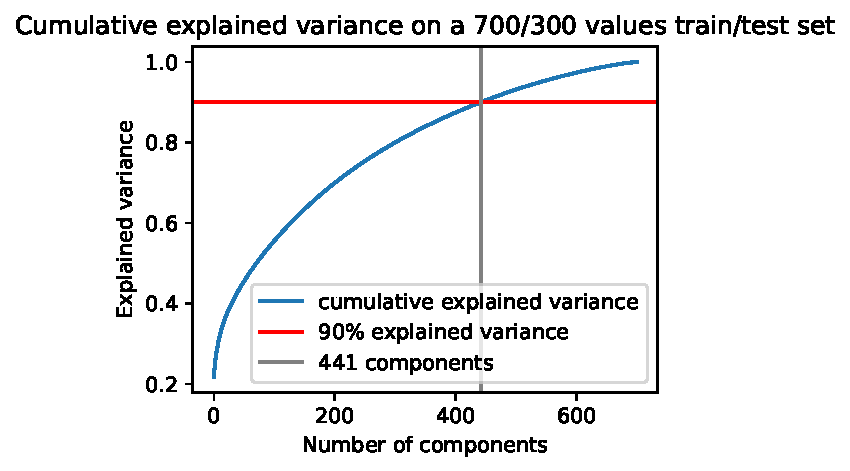
\includegraphics[width=7cm]{images/Eigendocs/Eval-Params/cumulative_explained_variance.pdf}}}%
    \qquad
    \subfloat[\centering The reconstruction error \ac{rmse} calculated for different values of $m$. Around 13 is an "elbow" point.]
    {{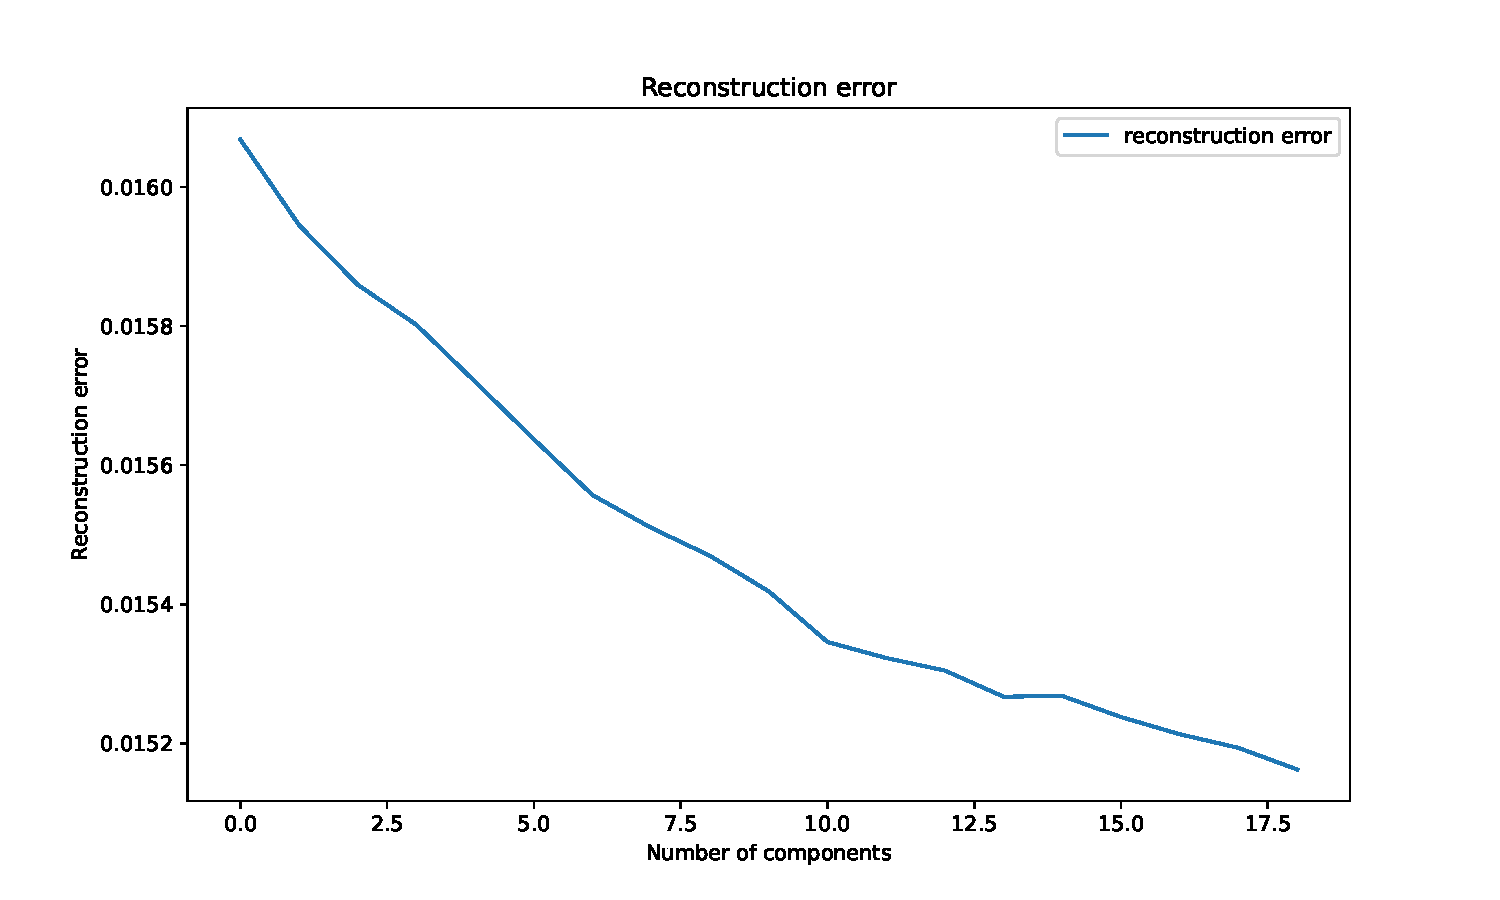
\includegraphics[width=7cm]{images/Eigendocs/Eval-Params/reconstruction error_eigendocs.pdf} }}%
    \caption[Approaches to find the number of \eigenfaces{}]{Two approaches in the literature to determine the number of \eigenfaces{} $m$ used to compress the input images.}%
    \label{fig:det_n_comp}%
\end{figure}

% calculation of eigenvectors of covariance matrix C
In order to reduce calculation complexity, $C$ is approximated.
% 1997
\citeauthor{eigenfaces1997} propose the approximation $\textbf{C} \simeq \frac{1}{N}\sum_{k=1}^{N}\textbf{x}_{k}\textbf{x}_{k}^{T} = \frac{1}{N}\textbf{X}\textbf{X}^{T}$, 
with $\textbf{X} = \left[ \textbf{x}_{1}, \textbf{x}_{2}, ..., \textbf{x}_{N} \right]$, $\textbf{x}_i \in \mathbb{R}^{n}$ \cite{eigenfaces1997}.

Finding the eigenvectors of $\textbf{X}\textbf{X}^{T}$ is still computationally expensive, since $\textbf{X}\textbf{X}^{T}$ is a $n$ by $n$ matrix.
According to \citeauthor{eigenfaces1997}, the eigenvectors of $\textbf{X}\textbf{X}^{T}$ can be calculated by using the eigenvectors of $\textbf{X}^{T}\textbf{X}$.
The eigenvalues $\textbf{e}_i \in \mathbb{R}^{n}$ of $\textbf{X}\textbf{X}^{T}$ can be derived from the eigenvectors $\textbf{v}_i \in \mathbb{R}^{N}$ of $\textbf{X}^{T}\textbf{X}$ by 
$\textbf{e}_i = \frac{1}{\sqrt{\lambda_i}}\textbf{X}\textbf{v}_i$ as discussed in more detail in \cite{eigenfaces1997}.
Hence, the problem is reduced to a $N$ by $N$ matrix, which is computationally less expensive to solve, since $N \ll n$.
Eigenvectors can be calculated using \ac{svd} \cite{eigenfaces1997}.
\ac{svd} is a method, which decomposes a matrix into the so-called left singular vector, the diagonal matrix and the right singular vector \cite{dim_reduction2021}. 
\ac{svd} facilitates the calculation of eigenvectors.

% classification/ compare
In the literature, face images are classified by comparing their position in the face space with those of already known faces \cite{eigenfaces1991}.
% performance 
According to \cite{eigenfaces1991}, this approach performs well on datasets with little variation in pose, lighting and facial expression.
However, \Citeauthor{eigenfaces1997} state, that the performance deteriorates if the variations increase since the changes introduce a bias 
that makes the distance function used to make classifications a no longer reliable measure.


\section{Clustering}\label{sec:clustering}

Clustering is used in a variety of domains to group data into meaningful subclasses \cite{OPTICS2013, OPTICS2014, OPTICS_kMeans_2016}.
According to \citeauthor{OPTICS2013} and \citeauthor{clusteringDocs2020}, common domains include anomaly detection, noise filtering, document clustering and image segmentation. 
The objective is to find clusters, which have a low inter-class similarity and a high intra-class similarity \cite{OPTICS2013}.
The similarity is measured by a distance function, which is dependent on the data type. 
Common distance functions are the Euclidean distance, the Manhattan distance and the Minkowski distance \cite{OPTICS_kMeans_2016}.

There are multiple clustering techniques, which can be divided into four categories \cite{OPTICS2016}: 
\begin{itemize}
    \item \textbf{Hierarchical clustering}:
    Algorithms, that create spherical or convex-shaped clusters, possibly naturally occurring. 
    A terminal condition has to be defined beforehand.
    Examples include CLINK, SLINK \cite{OPTICS2014} and \ac{optics} \cite{OPTICS2013}.

    \item \textbf{Partitional based clustering}: 
    Algorithms, that partition the data into $k$ clusters, $k$ is given apriori.
    Clusters are shaped in a spherical manner, are similar in size and not necessarily naturally occurring.
    KMeans is a popular example of a partitional-based clustering algorithm.

    \item \textbf{Density based clustering}:
    Density is defined as the number of objects within a certain distance of each other \cite{OPTICS_kMeans_2016}.
    The resulting clusters can be of arbitrary shape and size.
    The algorithm usually chooses the optimal number of clusters given the input data.
    However, some algorithms are sensitive to input parameters, such as radius, minimum number of points and threshold.
    Popular examples are \ac{dbscan} and \ac{optics}.
    
    \item \textbf{Grid based clustering}:
    Similar to density-based clustering, but according to \citeauthor{OPTICS2016} better than density-based clustering.
    Examples include flexible grid-based clustering \cite{OPTICS2014}.
    
\end{itemize}

Multiple approaches listed below use the term \textit{$\varepsilon$-neighbourhood}, which is defined as the set of all objects within a certain distance $\varepsilon$ of a given object \cite{OPTICS2013}.
In other words: $N_\varepsilon (x) = \left\{ y \in X | dist(x,y) \le \varepsilon, y \neq x \right\}$, $\varepsilon$ being the so-called generating distance.


%\subsection{KMeans}\label{subsec:kmeans}

KMeans partitions the data into $k \in \mathbb{N}$  clusters, $k$ is given apriori \cite{OPTICS_kMeans_2016,clusteringDocs2020}. %
First, $k$ centroids, i. e. cluster centres, are randomly initialized.
Then, the objects are assigned to the closest centroid.
Afterwards, the centroids are updated by calculating the mean of the assigned objects.
The process is repeated until the terminating condition, for instance, no more change in the clusters, is met \cite{OPTICS_kMeans_2016}.
By iteratively reassigning the objects to the closest centroid and updating the centroids, 
the algorithm minimizes the within-cluster sum of squared errors $E$, i. e. the sum of squared (Euclidean) distances between objects in a cluster and their centroid $\mu_{i}$, 
calculated in \autoref{eq:kmeans-error} from \cite{OPTICS_kMeans_2016}, 
where $C_{i}$ is the $i$-th cluster.

\begin{equation}
    E = \sum_{i=1}^{k} \sum_{x \in C_{i}}\left\|x-\mu_{i}\right\|^{2}
\label{eq:kmeans-error}
\end{equation}

\citeauthor{OPTICS_kMeans_2016} claim, that KMeans does not identify outliers.


\subsection{\acs*{dbscan}}\label{subsec:dbscan}

The clusters identified by \ac{dbscan} have a high density and are separated by low-density regions \cite{OPTICS_kMeans_2016}.
In order to create clusters of minimum size and density, \ac{dbscan} distinguishes between three types of objects \cite{OPTICS_kMeans_2016}:

\begin{itemize}
    \item \textbf{Core objects}: 
    An object $x$ with at least $minPts \in \mathbb{N}$ objects in its $\varepsilon$-neighbourhood $N_\varepsilon(x)$, i.e.\ $| N_\varepsilon (x) | \geq minPts$ is true \cite{OPTICS2013}.

    \item \textbf{Border objects}: 
    An object with less than $minPts$ objects in its $\varepsilon$-neighbourhood, which is in the $\varepsilon$-neighbourhood of a core object.

    \item \textbf{Noise objects}: 
    An object, which is neither a core object nor a border object.
\end{itemize}

\citeauthor{OPTICS_kMeans_2016} define $y \in X$ as \textit{directly density reachable} from $x \in X$, if $y$ is in the $\varepsilon$-neighbourhood of core object $x$ \cite{OPTICS_kMeans_2016}.
Moreover, a point $y \in X$ is \textit{density reachable} from $x \in X$, if there is a chain of objects $x_1, ..., x_n$ with $x_1 = x$ and $x_n = y$, 
which are directly density reachable from each other as displayed in \autoref{fig:density_reachable} \cite{OPTICS_kMeans_2016}.

\begin{figure}[!htb] % htp = hier (h), top (t), oder auf einer eigenen Seite (p).
    \centering
    \includesvg[width=0.2\textwidth]{images/density_reachable}
    \caption[Density reachability]{Density reachability cf. \cite{OPTICS1999}.
    The object $y \in X$ is density reachable from $x \in X$, since it exists a chain of directly density reachable objects between $x$ and $y$.
    }
    \label{fig:density_reachable}
\end{figure}

The objects $x \in X$ and $y \in X$ are said to be \textit{density connected}, if there is an object $o$, from which both $x$ and $y$ are density reachable \cite{OPTICS_kMeans_2016}.
Density connectivity is visualized in \autoref{fig:density_connected}.

\begin{figure}[!htb] % htp = hier (h), top (t), oder auf einer eigenen Seite (p).
    \centering
    \includesvg[width=0.2\textwidth]{images/density_connected}
    \caption[Density connectivity]{Density connectivity cf. \cite{OPTICS1999}.
    The objects $x$ and $y$ are density connected since there is an object $o$, from which both $x$ and $y$ are density reachable.
    }
    \label{fig:density_connected}
\end{figure}

The \ac{dbscan} algorithm starts by labeling all objects as core, border or noise points.
Then, it eliminates noise points and links all core points, which are within each other's neighbourhood \cite{OPTICS_kMeans_2016}.
Groups of connected core points form a cluster.
In the end, every border point is assigned to a cluster.
The non-core point cluster assigning is non-deterministic \cite{OPTICS2013}.
This algorithm creates clusters as a maximal set of density-connected points \cite{OPTICS_kMeans_2016}.

According to \citeauthor{OPTICS_kMeans_2016}, \ac{dbscan} can identify outliers or noise.
However, the algorithm is sensitive to the input parameters $minPts$ and $\varepsilon$ and has difficulties distinguishing closely located clusters \cite{OPTICS_kMeans_2016}.
Moreover, if one wants to obtain hierarchical clustering, one has to run the algorithm multiple times with different $\varepsilon$, which is expensive in terms of memory usage \cite{OPTICS2013}.
According to \citeauthor{clusteringDocs2020}, \ac{dbscan} is affected by the curse of dimensionality.
Since \ac{dbscan} relies on nearest neighbour queries and these become less meaningful in high dimensions, i.e.\ distances become difficult to interpret, 
the quality and accuracy of the results decline with increasing dimensionality \cite{clusteringDocs2020}.
\citeauthor{clusteringDocs2020} found that their \ac{dbscan} model assigns most objects noise when the dimensionality is sufficiently large.


\subsection{\acs*{optics}}\label{subsec:optics}

\ac{optics} does not return an explicit clustering, but rather a density-based clustering structure of the data, 
which is equivalent to repetitive clustering for a broad range of parameters \cite{OPTICS1999}.
\citeauthor{OPTICS1999} claim that real-world datasets cannot be described by a single global density, since they often consist of different local densities, 
as displayed in \autoref{fig:diff_density_cluster}.

\begin{figure}[!htb] % htp = hier (h), top (t), oder auf einer eigenen Seite (p).
    \centering
    \includesvg[width=0.4\textwidth]{images/diff_density_cluster}
    \caption[Clusters with different densities]{Clusters with different densities cf. \cite{OPTICS1999}.
    Since $C_1$ and $C_2$ have different densities than $A$ and $B$, a clustering algorithm using one global density parameter would detect the clusters $A$, $B$ and $C$, 
    rather than $A$, $B$, $C_1$ and $C_2$ .
    }
    \label{fig:diff_density_cluster}
\end{figure}

Opposed to \ac{dbscan}, \ac{optics} is able to detect clusters of varying densities \cite{OPTICS2014}.
\ac{optics} produces an order of the elements according to the distance to the already added elements \cite{OPTICS2014, OPTICS2013}:
The first element added to the order list is arbitrary.
%$\varepsilon$ defines the neighbourhood radius, i.e.\ the maximum distance between two elements, which are still considered to be in the same neighbourhood \cite{OPTICS_kMeans_2016}.
The order list is iteratively expanded by adding the element of the $\varepsilon$-neighbourhood to the order list, which has the smallest distance to any of the elements already in the order list.
Hence, clusters with higher density, i.e.\ lower $\varepsilon$, are added first (prioritized) \cite{OPTICS_kMeans_2016, OPTICS1999}.
When there are no more elements in the $\varepsilon$-neighbourhood to add, the process is repeated for the other clusters.
The non-core point cluster assigning is non-deterministic \cite{OPTICS2013}.

\begin{equation}
    RD(y) = \left\{
    \begin{array}{ll}
    \textrm{NULL} & \, \textrm{if |}N_\varepsilon (x)| < minPts \\
    max(core\_dist(x), dist(x,y)) & \, \textrm{otherwise} \\
    \end{array}
    \right. 
    \label{eq:optics-reachability-distance}
\end{equation}

\ac{optics} saves the reachability distance $RD(y)$, as calculated in \autoref{eq:optics-reachability-distance} from \cite{OPTICS2013},
with core distance $core\_dist$ being the minimal distance $\varepsilon^{min}$ such that $| N_{\varepsilon^{min}} (x) | \geq minPts$ 
(i.e.\ the distance to the $minPts^{th}$ point in $N_\varepsilon$) or NULL else, 
of each element $y$ to its predecessor $x$ in the order list and thus, 
a representation of the density necessary to keep two consecutive objects $x$ and $y$ in the same cluster \cite{OPTICS2013}.
If $\varepsilon < RD(y)$, then $y$ is not density reachable from any of its predecessors and thus, 
one can determine whether two points are in the same cluster for the information saved by \ac{optics} \cite{OPTICS2013, OPTICS1999}.
If the core distance of an element is not NULL, i.e.\ it is a core object, and it is not density reachable from its predecessors, it is the start of a new cluster \cite{OPTICS1999}.
Otherwise, the element is a noise point \cite{OPTICS1999}.
According to \citeauthor{OPTICS2013}, the algorithm builds a spanning tree, which enables obtaining the clusters for a given $\varepsilon$ by returning the connected components 
of the spanning tree after omitting all edges with $\varepsilon < RD(y)$ \cite{OPTICS2013}.
The relationship between $\varepsilon$, cluster density and nested density-based clusters is displayed in \autoref{fig:nested_density_cluster}.

% nested clusters, eps, fixed minPts
\begin{figure}[!htb] % htp = hier (h), top (t), oder auf einer eigenen Seite (p).
    \centering
    \includesvg[width=0.5\textwidth]{images/nested_density_cluster.svg}
    \caption[Relationship between $\varepsilon$, cluster density and nested density-based clusters]
    {The relationship between $\varepsilon$, cluster density and nested density-based clusters cf. \cite{OPTICS1999}.
    For a constant $minPts$, clusters with higher density such as $C_1$, $C_2$ and $C_3$, i.e.\ a low $\varepsilon_2$ value, 
    are completely contained in lower density clusters such as $C$ given $\varepsilon_1 > \varepsilon_2$.
    This idea forms the basis of \ac{optics} of expanding clusters iteratively and thus, 
    enables the detection of clusters for a broad range of neighbourhood radii $0 \le \varepsilon_i \le \varepsilon$.
    }
    \label{fig:nested_density_cluster}
\end{figure}

This procedure enables the extraction of clusters for arbitrary $0 \le \varepsilon_i \le \varepsilon$ \cite{OPTICS_kMeans_2016, OPTICS1999}.
According to \citeauthor{OPTICS2013}'s work, even though the clustering algorithm is expensive, the extraction only needs linear time.
According to \cite{OPTICS1999}, the algorithm yields good results if the input parameters $minPts$ and $\varepsilon$ are "large enough" and thus, the algorithm is rather insensitive to the input parameters.

% effect of eps (reachability plot)
The smaller $\varepsilon$ is chosen, the more objects will be identified as noise and thus, the algorithm will not identify clusters with low density, 
since some objects only become core objects for a larger $\varepsilon$ \cite{OPTICS1999}.
According to \citeauthor{OPTICS1999}, the optimal value for $\varepsilon$ creates one cluster for most of the objects with respect to a constant $minPts$,
since information about all density-based clusters for $\varepsilon_i < \varepsilon$ is preserved.
\citeauthor{OPTICS1999} present a heuristic for choosing $\varepsilon$ based on the expected $k$-nearest neighbour distance \cite{OPTICS1999}.

% effect of minPts (reachability plot)
High values for $minPts$ smoothen the reachability curve, even though the overall shape stays roughly the same \cite{OPTICS1999}.
According to \citeauthor{OPTICS1999}, the optimal value for $minPts$ is between 10 and 20.



\section{Database Elasticsearch}\label{sec:db}

% introduction, users
\databaseName{} is a widely used non-relational database, which was designed to store and perform full-text search on a large corpus of unstructured data \cite{Elasticsearch2017}.
This open-source distributed document-driven database system is built in Java and is based on the Apache Lucene (Java) library for high-speed full-text search \cite{Elasticsearch2017, Elasticsearch2019}.
According to \citeauthor{Elasticsearch2019}, \databaseName{} provides Wikipedia's full-text search and suggestions as well as Github's code search and Stack Overflow's geolocation queries and related questions.
It enables near real-time search by index refreshing periods of one second.
Needless to say, \databaseName{} is qualified to handle Big Data.

% structure
\databaseName{} is a document store, which stores schemaless key-value pairs called documents \cite{flask2018}.
The documents are stored in logical units, so-called indices.
% index
As stated by \citeauthor{Elasticsearch2019} and \citeauthor{Elasticsearch2017}, the indices are structured similarly to Apache Lucene's inverted index format.
An index can be spread into multiple nodes.
A node is a single running instance of \databaseName{} \cite{Elasticsearch2019}.
An index is divided into one or more shards, which can be stored on different servers and enable parallelization.
% Replicas
Replicas are copies of shards, which create redundancy and thus, ensure availability. %\cite{Elasticsearch2019}.

% document
The documents are saved in a \ac{json} format \cite{Elasticsearch2017}.
A document's fields and field types are defined by the user when initializing the database index.
By default, every field of a document is indexed and searchable \cite{Elasticsearch2019}.

% query (endpoints)
% get: search id
By specifying the unique \texttt{\_id} of a document and the database \texttt{index}, it is possible to retrieve a specific document from the database using the \texttt{GET \ac{api}}.
The query is real-time by default.
The parameters \texttt{\_source\_excludes} or \texttt{\_source\_includes} can be used to define the structure of the response \cite{Elasticsearch-get}.

% full-text search
The keyword used when performing a full-text search is \texttt{match}.
To query for a specific value, one has to specify the \texttt{<field>} of interest and the query value.

\databaseName{} preprocesses the query value before starting the search \cite{Elasticsearch-text-analyser}.
The default preprocessing steps of the so-called default analyzer include tokenization and lowercasing \cite{Elasticsearch-text-analyser}. 
Omitting stop words is disabled by default, but it is possible to provide custom stop words or use the English stop word list \cite{Elasticsearch-text-analyser}.
It is possible to create custom tokenizers, which split the query value into tokens of a certain maximum length.

Another useful feature of \databaseName{} is the multi-term synonym expansion.
When the user queries a specific phrase \databaseName{} expands the query to include synonyms of the query terms \cite{Elasticsearch-synonyms}.
The maximum number of expansion terms is set to 50 by default but can be configured by the user \cite{Elasticsearch-match}.
By default, the multi-terms synonym expansion option is enabled.

\databaseName{} also provides the option to perform fuzzy matching instead of exact search.
By enabling the fuzzy matching option, a \databaseName{} query consisting of for instance, \textit{Bahama} returns documents that contain the word \textit{Bahamas}.
By default, this option is not enabled but can be enabled and configured individually by the user \cite{Elasticsearch-match}.


% knn-search
Another search option of \databaseName{} is the \ac{knn} search.
The return value of a \ac{knn} search is the \texttt{k} nearest neighbours in terms of a certain distance function of a query vector \cite{Elasticsearch-kNN-HNSW}.
The query is a dense vector of the same dimension as the vectors stored in the database.
A \ac{knn} search either returns the exact brute-force nearest neighbours or 
an approximation of the nearest neighbours calculated by the \ac{hnsw} algorithm \cite{Elasticsearch-kNN-HNSW, Elasticsearch-knn}.
\ac{hnsw} is a graph-based algorithm \cite{Elasticsearch-kNN-HNSW}.
The term \texttt{navigable} refers to the graphs used, which are graphs with (poly-)logarithmic scaling of links traversed during greedy traversal concerning the network size \cite{Elasticsearch-kNN-HNSW}.
The idea of a \texttt{hiercharical} algorithm is to create a multilayer graph, grouping links according to their link length, as displayed in \autoref{fig:hnsw-layer}. 
The search starts on the uppermost layer, i.e. the layer containing the longest links, greedily traversing the layer until reaching the local minimum.
It uses this local minimum as the starting point at the next lower layer and the process is repeated until the lowest layer is reached \cite{Elasticsearch-kNN-HNSW}.
The layers of the graph are built incrementally, and a neighbour selection heuristic, as depicted in \autoref{fig:hnsw-heuristic}, not only creates links between close elements, 
but also between isolated clusters to ensure global connectivity \cite{Elasticsearch-kNN-HNSW}.

\begin{figure}[htp] % htp = hier (h), top (t), oder auf einer eigenen Seite (p).
    \centering
    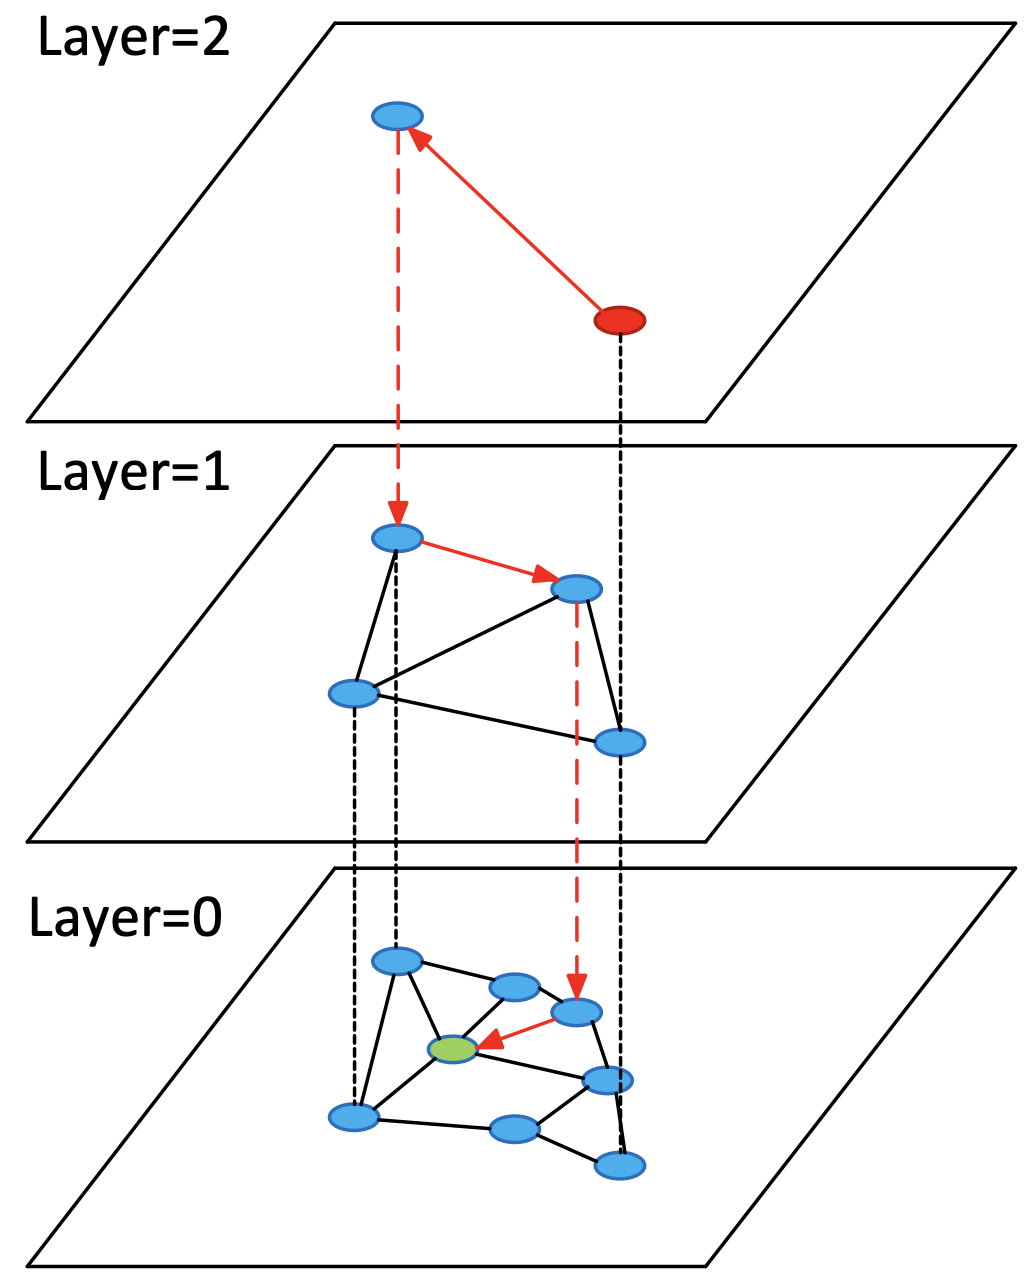
\includegraphics[width=0.3\textwidth]{images/Elasticsearch/HNSW-layer.png}
    \caption[Structure of \ac{hnsw} layers]{Structure of \ac{hnsw} layers from \cite{Elasticsearch-kNN-HNSW}.
    The search starts on the uppermost layer, i.e. the layer containing the longest links, greedily traversing the layer until reaching the local minimum.
    The local minimum is used as the starting point at the next lower layer and the process is repeated until the lowest layer is reached.
    }
    \label{fig:hnsw-layer}
\end{figure}

\begin{figure}[htp] % htp = hier (h), top (t), oder auf einer eigenen Seite (p).
    \centering
    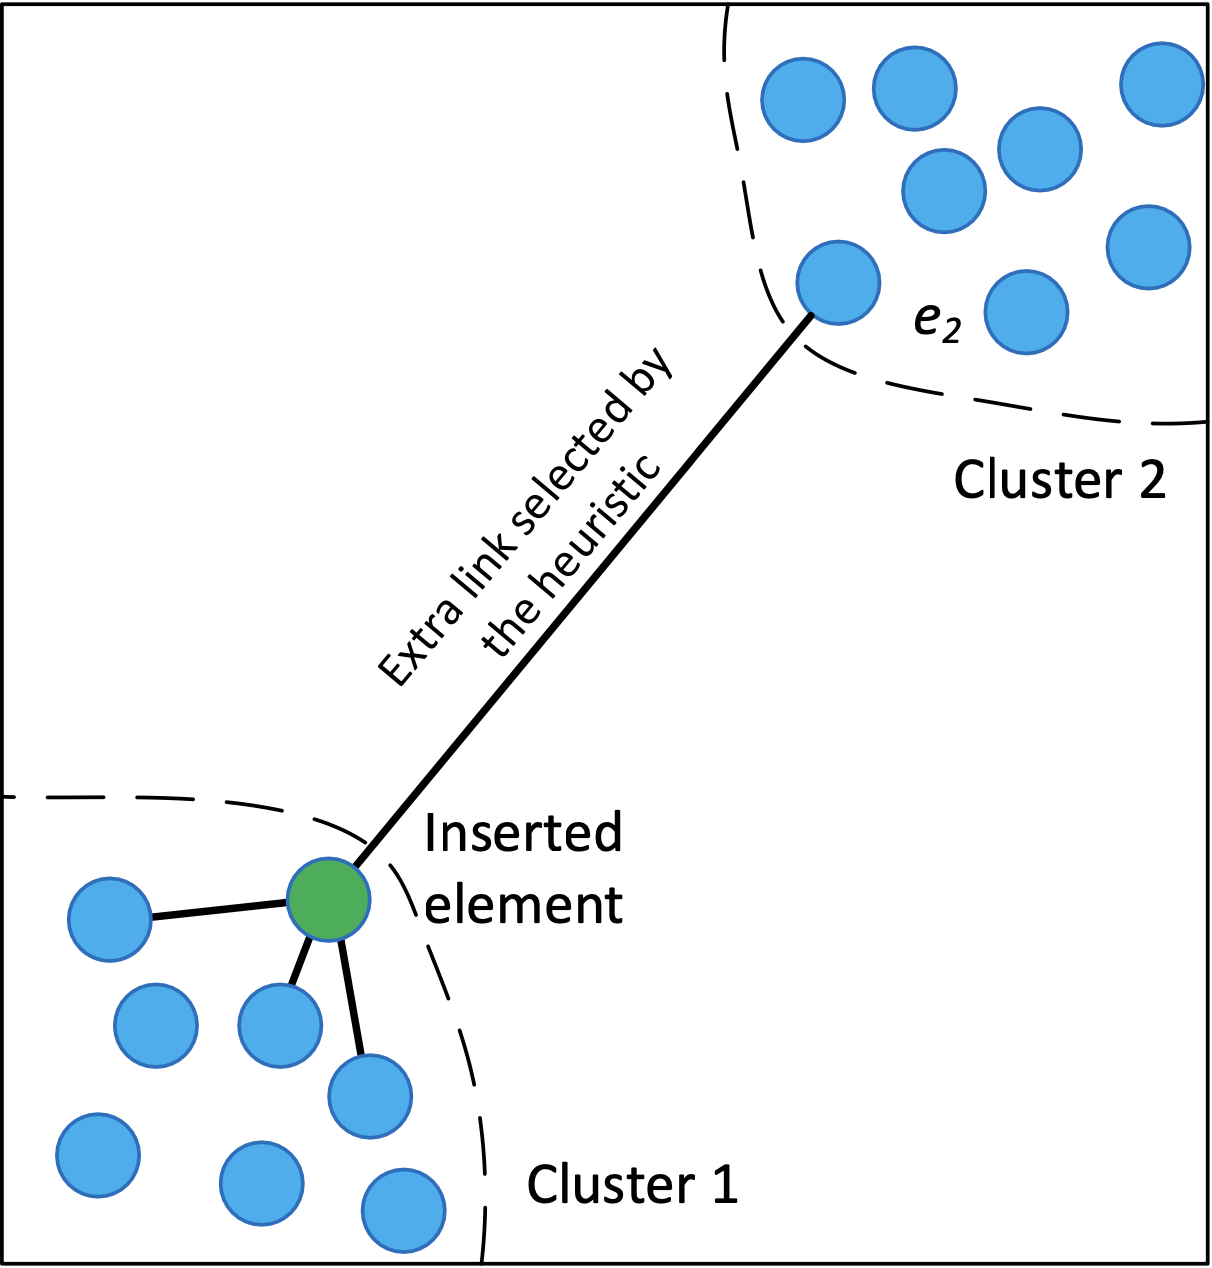
\includegraphics[width=0.3\textwidth]{images/Elasticsearch/HNSW-neighbour-selection-heuristic.png}
    \caption[Neighbour selection heuristic of \ac{hnsw}]{Neighbour selection heuristic of \ac{hnsw} from \cite{Elasticsearch-kNN-HNSW}.
    The heuristic creates diverse links, i.e. links between close elements (e.g., green circle and elements in cluster 1) 
    and between isolated clusters (e.g., green circle and $e_2$) to ensure global connectivity.
    }
    \label{fig:hnsw-heuristic}
\end{figure}

In order to perform \ac{knn} search on a \texttt{<field>} it has to be of type \texttt{dense\_vector}, indexed and a \texttt{similarity} measure has to be defined when initializing the database \cite{Elasticsearch-knn}.
\databaseName{}'s \ac{knn} implementation not only allows literal matching on search terms but also semantic search \cite{Elasticsearch-knn}.

Besides \databaseName{}, the elastic stack offers other tools, for instance, Kibana, which provides a user interface to manage different models.
After saving a model in Kibana, it is possible to create a text embedding ingest pipeline, which embeds new documents or reindexes existing documents \cite{Elasticsearch-knn-embedding}.



\section{\flask{}}\label{sec:BE_flask}

% introduction
\flask{} is open source and written in Python by Armin Ronancher in 2004 \cite{flask2015, mvc_flask2019}.
According to \citeauthor{flask_book2015} and \citeauthor{mvc_flask2019}, \flask{} is one of the most popular Python web frameworks.
It provides powerful libraries for core functionality such as routing, templating, and \ac{http} request parsing \cite{flask_book2015}.
It is extensible and thus, can be extended with additional plugins without affecting the internal structure of the existing system \cite{flask2015}.

% technical details
\flask{} uses the Jinja Template Engine for template files including \ac{html} pages,
whereas static files such as \ac{css} files are handeled using the Werkzeug WSGI toolkit \cite{flask2015}.
According to \citeauthor{flask2015}, Jinja is modeled after the Django template system.
Werkzeug implements, for instance, requests and response objects \cite{mvc_flask2019}.

% initialization
All requests received from clients are passed to an instance of the \flask{} application \cite{flask_book2018}.
Hence, the first step is to create an instance of the \flask{} class, such as done in \lst{lst:flask_app_init}.

\begin{listing}[htp]
    \begin{minted}{python3}
    app = Flask(__name__)
    \end{minted}
    \caption[Initialization of \flask{} application instance]{Initialization of \flask{} application instance.
    }
    \label{lst:flask_app_init}
\end{listing}

% routing
Clients send requests to the web server, which passes them to the \flask{} application instance.
The queries are then routed to the corresponding functions.
Routing is the process of mapping \ac{url} paths to functions \cite{flask_book2018}.
To define a route, the \texttt{route} decorator is used as displayed in \lst{lst:flask_routing}.

\begin{listing}[htp]
    \begin{minted}{python3}
    @api.route('/documents/<id>', endpoint='document')
    class Document(Resource):
        def get(self, id):
            elastic_search_client = Elasticsearch(CLIENT_ADDR)
            return query_database.get_doc_meta_data(elastic_search_client, 
                doc_id=id)
    \end{minted}
    \caption[Routing using \flask{}]{Exemplartary definition of a function to display routing with \flask{}.
    The \texttt{route} decorator is used to define the \ac{url} path.
    }
    \label{lst:flask_routing}
\end{listing}

\acs{url} can contain dynamic components, which are enclosed in \texttt{<>} angle brackets.
The values of these components are passed to the function as arguments \cite{flask_book2018}.
By default, dynamic components are of type \texttt{string}.
However, other types including \texttt{int} and \texttt{float} are supported \cite{flask_book2018}.

% dev server
During development, the \flask{} application can be run using \texttt{flask run} to start the built-in development web server \cite{flask_book2018}.
By enabling debug mode, the server automatically reloads the application when changes are detected \cite{flask_book2018}.

% endpoints
An endpoint is a class with certain methods, which can be accessed using \ac{http} requests.
Every endpoint can have multiple decorators, including \texttt{GET}, \texttt{POST}, \texttt{PUT} and \texttt{DELETE} \cite{flask2018}.
The \texttt{GET} method is used to retrieve data from the server, whereas the other methods are used to either insert, update or delete data.


\section{\angular{}}\label{sec:FE_angular}

\angular{} is a framework for building web applications.
It uses Node.js and TypeScript.
Usually, the source code is structured into different modules, including components and services.
Components are used to define the appearance of the application, while
service modules contain the logic of the application and communicate with the backend.

% creating applications
\angular{} applications are created using the \texttt{ng new NAME} command line interface \cite{angular_book2018}.
This command creates a skeleton, which can be customized to meet the needs of the application.
By running \texttt{ng serve} the application can be served locally.